\documentclass[a4paper,11pt]{article}

%%%%%%%%%%%%%%%%%%%%%%%%%%%%%%%%%%%%%%%%%%%%%%%%%%%%%%%%%%%%%%%%%%%%%%%%
% Paquetes utilizados
%%%%%%%%%%%%%%%%%%%%%%%%%%%%%%%%%%%%%%%%%%%%%%%%%%%%%%%%%%%%%%%%%%%%%%%%

% Gráficos complejos
\usepackage{graphicx}
\usepackage{caption}
\usepackage{subcaption}
\usepackage{placeins}

% Soporte para el lenguaje español
\usepackage{textcomp}
\usepackage[utf8]{inputenc}
\usepackage[T1]{fontenc}
\DeclareUnicodeCharacter{B0}{\textdegree}
\usepackage[spanish]{babel}

% Código fuente embebido
\usepackage{listings}

% PDFs embebidos para el apéndice
\usepackage{pdfpages}

% Matemáticos
\usepackage{amssymb,amsmath}

% Tablas complejas
\usepackage{multirow}

% Formato de párrafo
\setlength{\parskip}{1ex plus 0.5ex minus 0.2ex}

%%%%%%%%%%%%%%%%%%%%%%%%%%%%%%%%%%%%%%%%%%%%%%%%%%%%%%%%%%%%%%%%%%%%%%%%
% Título
%%%%%%%%%%%%%%%%%%%%%%%%%%%%%%%%%%%%%%%%%%%%%%%%%%%%%%%%%%%%%%%%%%%%%%%%

% Título principal del documento.
\title{\textbf{Trabajo Práctico 2: Profiling y optimización}}

% Información sobre los autores.
\author{
  Andrés Gastón Arana, \textit{P. 86.203}                          \\
  \texttt{and2arana@gmail.com}                                     \\
  Sergio Matías Piano, \textit{P. 85.191}                          \\
  \texttt{smpiano@gmail.com}                                       \\ [2.5ex]
  \normalsize{2do. Cuatrimestre de 2012}                           \\
  \normalsize{66.20 Organización de Computadoras}                  \\
  \normalsize{Facultad de Ingeniería, Universidad de Buenos Aires}
}
\date{}

%%%%%%%%%%%%%%%%%%%%%%%%%%%%%%%%%%%%%%%%%%%%%%%%%%%%%%%%%%%%%%%%%%%%%%%%
% Documento
%%%%%%%%%%%%%%%%%%%%%%%%%%%%%%%%%%%%%%%%%%%%%%%%%%%%%%%%%%%%%%%%%%%%%%%%

\begin{document}

% ----------------------------------------------------------------------
% Top matter
% ----------------------------------------------------------------------
\thispagestyle{empty}
\maketitle

\begin{abstract}

  Este informe sumariza el desarrollo del trabajo práctico 2 de la materia
  Organización de Computadoras (66.20) dictada en el segundo cuatrimestre de
  2012 en la Facultad de Ingeniería de la Universidad de Buenos Aires. El mismo
  consiste en la optimización de un sistema de simulación con énfasis en el
  análisis de perfilado y aprovechamiento de cache.

\end{abstract}

\clearpage

% ----------------------------------------------------------------------
% Tabla de contenidos
% ----------------------------------------------------------------------
\tableofcontents
\clearpage


% ----------------------------------------------------------------------
% Desarrollo
% ----------------------------------------------------------------------
\part{Desarrollo}

\section{Algoritmo de implementación}

El sistema analizado simula la evolución de un ecosistema simplificado en un
planeta ficticio toroidal denominado Wator. Para hacerlo, mantiene una matriz
de \(32x32\), donde cada celda representa una unidad de espacio en la
superficie del planeta. La celda está representada por una estructura que
contiene datos acerca del animal que está alojado en ella (tiempo de vida,
hambre y tipo de animal), junto con un flag que marca, para cada iteración, si
la celda ya ha sido procesada o no.

Se inicializa al azar cada una de las celdas, de acuerdo a ciertos parámetros
de distribución de cada tipo de animal, y luego se simulan 1000 turnos de
evolución del ecosistema. En cada turno se procesa secuencialmente cada una de
las celdas de acuerdo al tipo de animal alojado en la celda y las reglas
propias del ecosistema. Al finalizar cada turno se imprime por pantalla o a un
archivo el estado del mapa.

\section{Profiling inicial} \label{sec:profinicial}

Primeramente se examinó el código y se eliminaron algunos problemas en la
estructura del programa. Particularmente se eliminaron las variables sin
utilizar y se unificaron las funciones \textit{choose\_fish} y
\textit{choose\_empty} en una única función: \textit{choose\_random}. Se
decidió hacer esta modificación dado que las funciones eran absolutamente
equivalentes, distinguiendose únicamente por el tipo de celda que buscaban en
el mapa, y unificándolas podemos tener un mejor resultado en el profiling a la
hora de analizar si la estrategia de procesamiento en la búsqueda es la más
adecuada a los parámetros de ejecución del sistema.

Se realizó un perfilado de la ejecución del programa utilizando la herramienta
\textit{gprof}. La mayor parte del tiempo de ejecución está concentrado en 3
funciones: \textit{choose\_random}, \textit{move\_to\_fish} y
\textit{move\_to\_empty}. Es en estas tres funciones que nos detendremos
inicialmente para analizar que propuestas de optimización pueden realizarse.

\section{Optimizaciones propuestas}

En base a los resultados del perfilado sumarizados en la sección~\ref{sec:profinicial}, se determinaron diversas alternativas para intentar mejorar la performance del sistema en la arquitectura detallada en el enunciado del trabajo práctico. En cada una de ellas se intentó cumplir con uno de los dos objetivos enunciados a continuación:

\begin{enumerate}

  \item Disminuir la cantidad de accesos a memoria principal y la tasa de falla
      en el cache de la arquitectura propuesta por el ejercicio.

  \item Disminuir la cantidad de operaciones necesarias para alcanzar la
      solución deseada.

\end{enumerate}

Decidimos priorizar el disminuir la tasa de fallas en el cache antes que la
cantidad de operaciones necesarias para calcular la solución. Esta decisión
está basada en el gran impacto que tienen los tiempos de acceso a memoria en el
tiempo de ejecución del programa. Cabe destacar que esta priorización no es
fija, sino que se evalua con criterio: si disminuir el miss rate en un
\(0.01\%\) implica realizar el doble de operaciones, quizás no se observe una
mejora en el tiempo de ejecución sino todo lo contrario.

En las siguientes secciones discutimos algunas de las optimizaciones
propuestas, ordenadas de menor a mayor complejidad, incluyendo los motivos que
podrían colaborar a obtener una mejora de performance así como las
consecuencias de su implementación que llevan a empeorar el tiempo de ejecución
del sistema. Seleccionaremos algunas de ellas para implementar sucesivamente
sobre el código del trabajo práctico y realizar las mediciones pertinentes para
confirmar o rechazar las predicciones propuesta, así como la eficiencia ganada
al tomarlas.

\subsection{Reemplazar variables por constantes}

\subsection{Actualizar flag de proceso en una única iteración}

\subsection{Recálculo de ubicaciones en interface de \textit{choose\_random}}

\subsection{Disminuir el tamaño por celda}

\subsection{Seleccionar nuevas estructuras de datos}


\section{Implementación de optmizaciones}

\section{Conclusiones}


\clearpage

\part{Apéndice}
\appendix

\section{Enunciado original}\label{sec:enunciado}
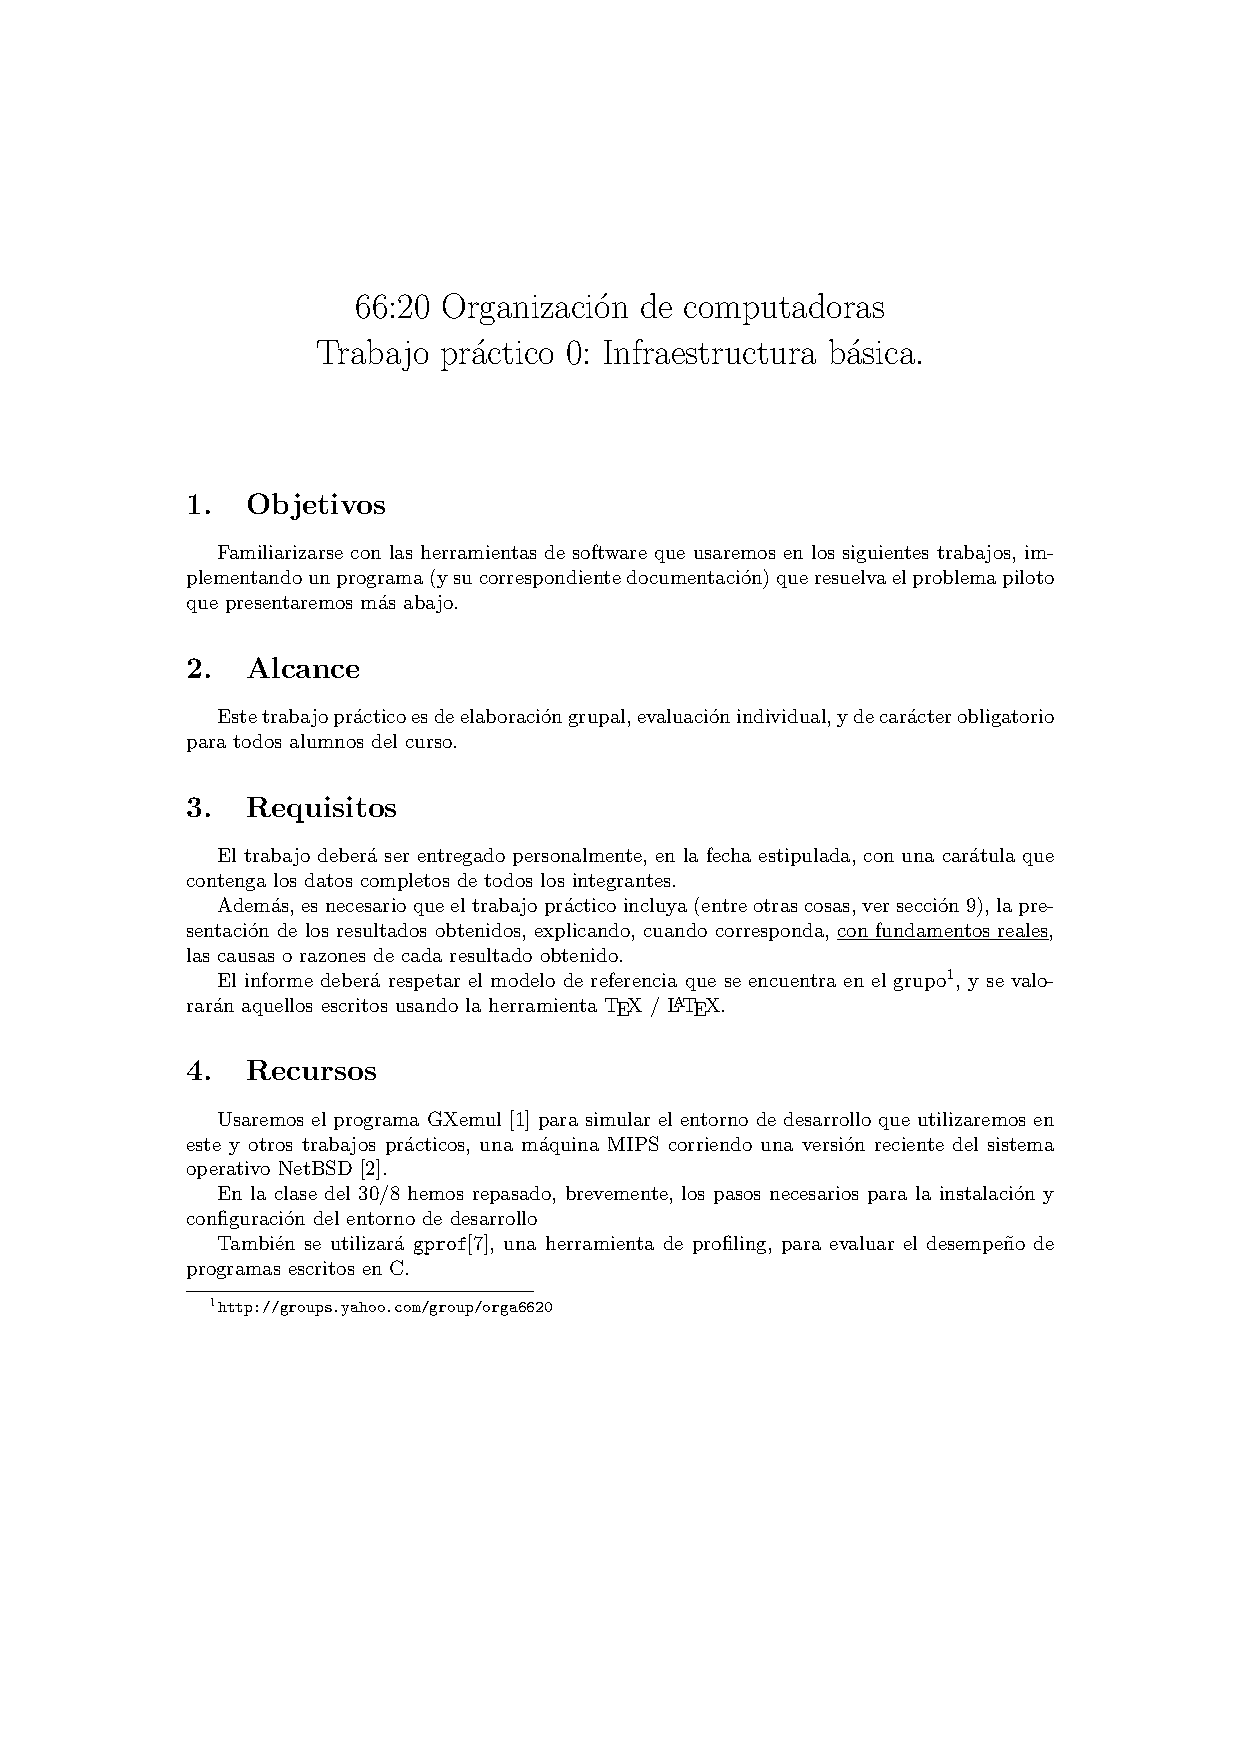
\includepdf[pages={-}]{docs/enunciado.pdf}

\clearpage
\section{README del material digital}\label{sec:readme}
\includepdf[pages={-}]{build/doc/README.pdf}

\clearpage
\section{Código fuente optimizado}\label{sec:source}
\clearpage
\definecolor{gray}{rgb}{0.5,0.5,0.5}
\lstset{title=\lstname,
  basicstyle=\footnotesize,
  showspaces=false,
  showstringspaces=false,
  breaklines=true,
  commentstyle=\color{gray},
  numbers=left,
  numberstyle=\tiny\color{gray},
  numbersep=5pt,
  frame=single
}

\lstinputlisting{source/wator.c}

\end{document}

